\label{tutorial}

\subsection{Quickstart}
{\small
\begin{lstlisting}[backgroundcolor=\color{grey},language=SQL]
java -jar lusql.jar -l quickstartIndex -q "select * from mytable" \
 -c "jdbc:mysql://dbhost/db?user=ID\&password=PASS"
\end{lstlisting}
}

Create a Lucene index called {\tt quickstartIndex} which indexes all the
fields of all the records in table {\tt mytable}, from database {\tt db}
on MySQL database host {\tt dbhost}, with user {\tt ID}, password {\tt PASS}. 



\subsection{Tutorial-by-example}

This tutorial uses four examples of progressively increasing complexity,
to present different aspects of LuSql functionality.
\begin{mlist}
\item In the first, a single table is queried using a simple SQL query to produce an
index.
\item In the second, a complex set of tables is queried with a join intensive SQL
query.
\item In the third, the second example is extended using per-record
subqueries, to include data from M:N tables.
\item In the fourth, the third example is extended using a {\tt
  DocFilter},
  and uses a field which contains the file system path to a text file whose
  full-text is read and indexed as an additional field.
\end{mlist}

The tutorial assumes a MySQL database, a Linux/Unix--like command-line
  environment, and uses 
  {\bf Luke}\footnote{\url{http://www.getopt.org/luke/}
}
or the {\em Lucene Index Toolbox} to validate the created indexes.
Luke is a Java application that allows - among many other useful things - the 
examination of Lucene indexes and the perusal of the {\tt Document}s and
  {\tt Field}s that the indexes contain.

A description of the hardware, operating system, Java versions, etc. used in
the tutorial can be found in \mbox{Appendix \ref{hardware}}.


\subsection{Example 1: Single table}
\label{example1}
Given the following table:
{\small
\begin{verbatim}
   mysql> describe Article;
   +--------------+-------------+------+-----+---------+-------+
   | Field        | Type        | Null | Key | Default | Extra |
   +--------------+-------------+------+-----+---------+-------+
   | id           | int(11)     | YES  |     | NULL    |       | 
   | articleTitle | varchar(64) | YES  |     | NULL    |       | 
   | abstract     | text        | YES  |     | NULL    |       | 
   | startPage    | varchar(16) | YES  |     | NULL    |       | 
   | journalTitle | text        | YES  |     | NULL    |       | 
   | issn         | char(12)    | YES  |     | NULL    |       | 
   | volumeNumber | varchar(32) | YES  |     | NULL    |       | 
   | volumeYear   | char(16)    | YES  | MUL | NULL    |       | 
   | issueNumber  | varchar(32) | YES  |     | NULL    |       | 
   +--------------+-------------+------+-----+---------+-------+
\end{verbatim}
   
\begin{verbatim}
   mysql> select count(id) from Article;
   select count(id) from Article;
   +-----------+
   | count(id) |
   +-----------+
   |   6409484 | 
   +-----------+
\end{verbatim}

\begin{verbatim}
   mysql> select count(id)  from Article where volumeYear > 2007;
   +-----------+
   | count(id) |
   +-----------+
   |       218 | 
   +-----------+
\end{verbatim}
}

Let's say we want to create a Lucene index, using the
{\tt StandardAnalyzer\footnote{
    \url{http://lucene.apache.org/java/2_3_1/api/org/apache/lucene/analysis/standard/StandardAnalyzer.html}
  }}, 
  and want all fields to be:
\begin{mlist}
\item
{\tt
        Field.Index.TOKENIZED\footnote{\url{http://lucene.apache.org/java/2_3_2/api/org/apache/lucene/document/Field.Index.html}{TOKENIZED}}
}

\item
{\tt
        Field.Store.YES\footnote{\url{http://lucene.apache.org/java/2_3_2/api/org/apache/lucene/document/Field.Store.html}{YES}}
}

\item {\tt Field.TermVector.YES\footnote{\url{http://lucene.apache.org/java/2_3_2/api/org/apache/lucene/document/Field.TermVector.html}{YES}
}
}
\end{mlist}

\noindent but we only want the records that have {\tt volumeYear} $>$  2007 and we
only want the first 100 records.

LuSql offers a ``test'' mode which does no indexing and does not create a Lucene
index, but instead prints the results of your SQL query.
This is to validate that your SQL query is valid, and for you to see if the
fields and their values returned by your query make sense.


Here is how you would invoke LuSql, assuming a Linux shell (bash)
 environment\footnote{In most Unix/Linux shell environments, the
 backslash ($\backslash$) denotes that the command is continued on the
 next line}:

{\small
\begin{lstlisting}[backgroundcolor=\color{grey},language=SQL,numbers=left]
java -jar lusql.jar  \(*@\label{java}@*)
 -q "select * from Article where  volumeYear >  2007" \(*@\label{q}@*)
 -c "jdbc:mysql://dbhost/db?user=ID&password=PASS"\ (*@\label{c}@*)
 -n  5  \(*@\label{n}@*)
 -l tutorial-1 \(*@\label{l}@*)
 -v \(*@\label{v}@*)
 -I 211 \(*@\label{I}@*)
 -t(*@\label{t}@*)
\end{lstlisting}
}



Explanation:
\begin{mlist}
  \item Line \ref{java}: invoke LuSql.
  \item Line \ref{q}: {\tt -q} SQL statement to be used.
  \item Line \ref{c}: {\tt -c} JDBC URL to use.
    Note that this may be different across different JDBC drivers.
  \item Line \ref{c}: {\tt -n} limit the number of records indexed, or, in
    this case ({\tt -t}) the number of records to print out.
  \item Line \ref{l}: {\tt -l} the directory for the Lucene index.
    If the directory does not exist, it will be created.
    If it exists, it will be overwritten (default).
  \item Line \ref{v}: {\tt -v} verbose output showing various attributes and
    a progress indicator.
    The default mode is to produce no console output.
  \item Line \ref{I}: {\tt -I} defines a single set of
    {\tt Field.Index}, {\tt Field.Store}, and {\tt Field.TermVector} values to
    be applied to all fields to be included in the Lucene {\tt Document}. 
    The {\tt -I} parameter has the form {\tt NNN} where the respective {\tt
      Field} attributes are defined as:\label{nnn}
{\small
\begin{verbatim}
       Index: Default:TOKENIZED (2)
        0:NO
        1:NO_NORMS
        2:TOKENIZED
        3:UN_TOKENIZED
       Store: Default:YES (1)
        0:NO
        1:YES
        2:COMPRESS
       Term vector: Default:YES (1)
        0:NO
        1:YES
        2:WITH_OFFSETS
        3:WITH_POSITIONS
        4:WITH_POSITIONS_OFFSETS
\end{verbatim}
}

Note that if neither {\tt -I} nor {\tt -i} is set, the default is: {\tt -I
  211}.  
  \item Line \ref{t}: {\tt -t} test mode
\end{mlist}

Example test ({\tt -t}) output for only 5 records\footnote{Appendix
  \ref{hardware} shows the test configuration for the indexing and DBMS
  hardware} (long lines are truncated with {\tt ...}):
{\small
%\begin{verbatim}
\begin{lstlisting}[backgroundcolor=\color{grey}]
> java -jar lusql.jar -q "select * from Article where volumeYear > 2007" \
  -c "jdbc:mysql://dbhost/db?user=USERID&password=PASSWORD"\
  -n 5 -l tutorial-1 -v -I 211 -t
Using sql:[select * from Article where volumeYear > 2007]
Using Analyzer:[org.apache.lucene.analysis.standard.StandardAnalyzer]
Using Stop Word FileName:[null]
Using Properties FileName:[null]                                                            
Using DB driver name:[com.mysql.jdbc.Driver]
Using DB URL:[jdbc:mysql://dbhost/db?user=USERID\&password=PASSWORD]
Using Lucene index:tutorial-1
Using Lucene index RAMBUFFER MBs:48.0 
Using multithreaded:true  
Using Test:true 
Using Field parameters:211
Using setting DB fetchsize=0 (see -m)
Using Num documents to add:5 
Using Lucene index directory:tutorial-1   
Opening Lucene index: tutorial-1
Opening MySQL connection 
Querying:select * from Article where volumeYear > 2007 
Test only: not indexing: SQL results  
> id=2486095; articleTitle=Complexation of io...; ...
> id=2486107; articleTitle=Microwave-assisted...; ...
> id=2486111; articleTitle=Diffraction effici...; ...
> id=2486116; articleTitle=The synthesis and...; ...
> id=2486119; articleTitle=Synthesis and phot...; ...
Closing JDBC: result set
Closing JDBC: statement
Closing JDBC: connection
*********** Elapsed time: 0 seconds 
\end{lstlisting}
%\end{verbatim}
}
\noindent Perusing the SQL query shows us that this is indeed what we want, so now we
invoke LuSql without the {\tt -t} test flag, and change the number of result
records to index from 5 to 100:
{\small 
%\begin{verbatim}
\begin{lstlisting}[backgroundcolor=\color{grey}]
> java -jar lusql.jar \
-q "select * from Article where volumeYear > 2007"\
-c "jdbc:mysql://dbhost/db?user=USERID&password=PASSWORD"\
-n 100 -l tutorial-1 -v -I 211
Using sql:[select * from Article where volumeYear > 2007]
Using Analyzer:[org.apache.lucene.analysis.standard.StandardAnalyzer]
Using Stop Word FileName:[null]
Using Properties FileName:[null]
Using DB driver name:[com.mysql.jdbc.Driver]
Using DB URL:[jdbc:mysql://dbhost/db?user=USERID&password=PASSWORD]
Using Lucene index:tutorial-1
Using Lucene index RAMBUFFER MBs:48.0
Using multithreaded:true
Using Test:false
Using Field parameters:211
Using setting DB fetchsize=0 (see -m)
Using Num documents to add:100
Using Lucene index directory:tutorial-1
Opening Lucene index: tutorial-1
Opening MySQL connection
Querying:select * from Article where volumeYear > 2007
Indexing
Threading: Queue size=60
Threading: # threads=20

Number of records added= 100

Optimizing index
  Closing index
  Optimizing index time: 0 seconds
Closing JDBC: result set
Closing JDBC: statement
Closing JDBC: connection
*********** Elapsed time: 7 seconds
>
\end{lstlisting}
%\end{verbatim}
}


%% As shown in the output, a number of parameters have implicit default
%% values.
%% We will examine some of these in the more advanced examples, as well
%% examining all command line arguments in Section \ref{cli}.

\subsubsection{Example 1 examined in Luke}
Here, we will use Luke to verify the index we just created.
\begin{mlist}

\item Figure \ref{luke_1_1} shows the index in the Luke {\tt Overview} panel.
  It shows the name of the index, the number of documents, the number of
  documents per field, etc.
  The number of documents, fields, etc., appear to be what we wanted.

\item Figure \ref{luke_1_2} shows the Luke {\tt Documents} panel, which allows for
  the perusal of individual documents and their fields.
  This is used to validate that the right records are in the index, and to check
  exactly how each field has been indexed.
  Hand checking this information with a query of the database validates
  that it is the right information.
  The {\tt Flags} indicating the Lucene storage parameters also appear to be
  what we expect. 

\item Figure \ref{luke_1_3} shows the Luke {\tt Search} panel which allows the user to
  formulate queries and apply them to the index.
  Note that the {\tt Analyzer} selected is the {\tt StandardAnalyzer}\footnote{\tt
    org.apache.lucene.analysis.standard.StandardAnalyzer} which matches the
  one we used in our indexing; the default
  {\tt Analyzer} for Luke is {\tt
    SimpleAnalyzer}\footnote{{\tt org.apache.lucene.analysis.standard.SimpleAnalyzer}}. 
  Using a different {\tt Analyzer} for indexing and querying may result in
  unpredictable (and undesirable) behaviour.
  The query returns the correct, and the correct number of, {\tt Documents}.
  Here is a validating\footnote{
    Caution must be applied when doing this kind of validation, as 
    differences in indexing in Lucene and the SQL database can cause
    significant differences in the type and number of results returned. 
    There is no 1:1 mapping of Lucene queries to SQL queries.
    That said, it is still useful to do this kind of validation querying,
    as long as you understand the results.}
  SQL query:\\
{\small 
\begin{lstlisting}[backgroundcolor=\color{grey}]
  mysql> select id from Article where volumeYear > 2007  \
     and abstract like "%ionic%" and journalTitle like "%pigments%"\
     and articleTitle like "%surfactants%";
   +---------+
   | id      |
   +---------+
   | 2486095 | 
   | 2486179 | 
   +---------+
\end{lstlisting}
}
    While this seems like a problem as the SQL query produces more results
    than Luke (id=2486095 matches what Luke tells us, but id=2486179 does
    not), deeper examination shows that the second id is the $110^th$ record
    returned by {\tt select count(id)  from Article where volumeYear > 2007},
    so it is not in our Lucene index, explaining why Luke does not show it.
\end{mlist}

%\begin{landscape}
  \begin{figure}
  \begin{center}
 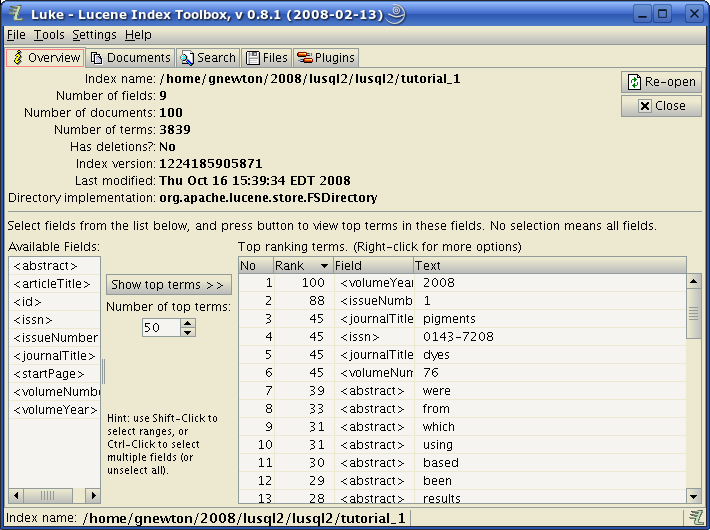
\includegraphics[width=\textwidth]{images/luke_1_1.png}
 % 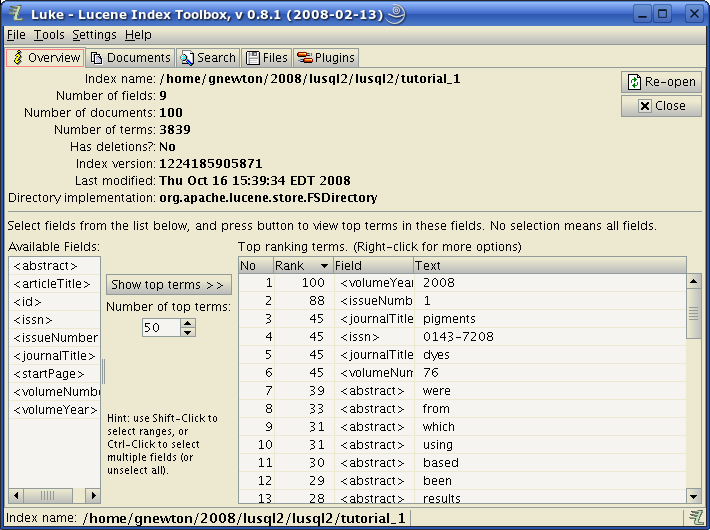
\includegraphics[height=\textwidth]{images/luke_1_1.png}
%  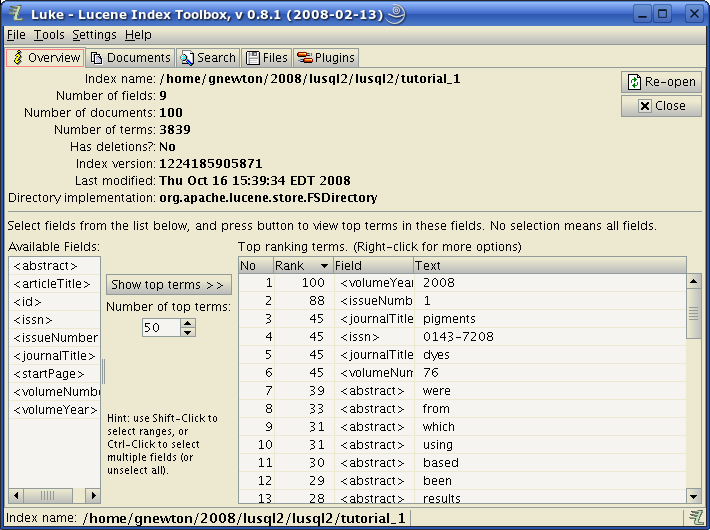
\includegraphics[width=16cm]{images/luke_1_1.png}
      \end{center}
  \caption{Example 1 in {\tt Luke}: Overview panel}
\label{luke_1_1}
\end{figure}

%\begin{landscape}
\begin{figure}
  \begin{center}
  % \scalebox{0.5}{
  %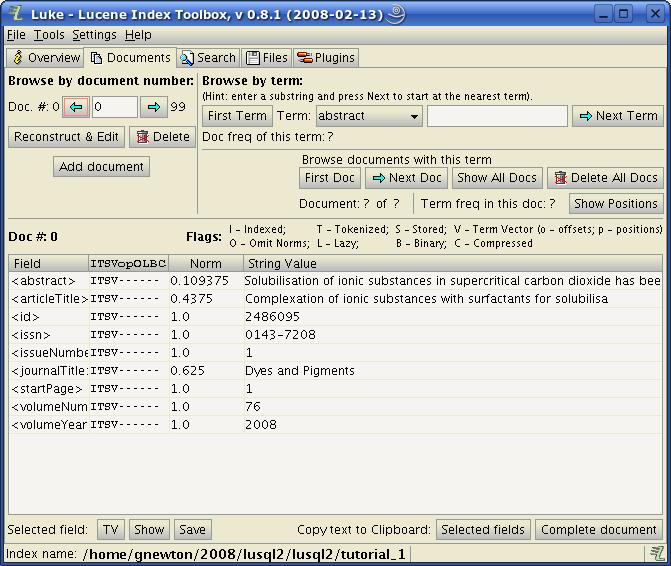
\includegraphics[height=\textwidth]{images/luke_1_2.png}
  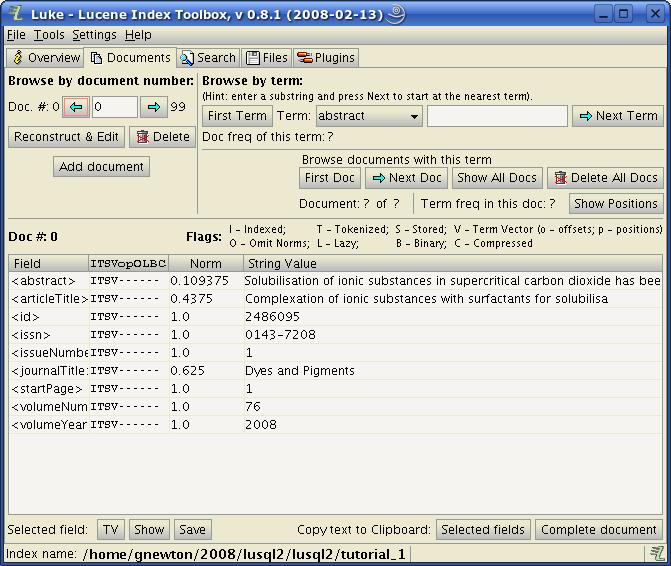
\includegraphics[width=\textwidth]{images/luke_1_2.png}
        % }
      \end{center}
  \caption{Example 1 in {\tt Luke}: Documents panel}
\label{luke_1_2}
\end{figure}

\begin{figure}
  \begin{center}
%    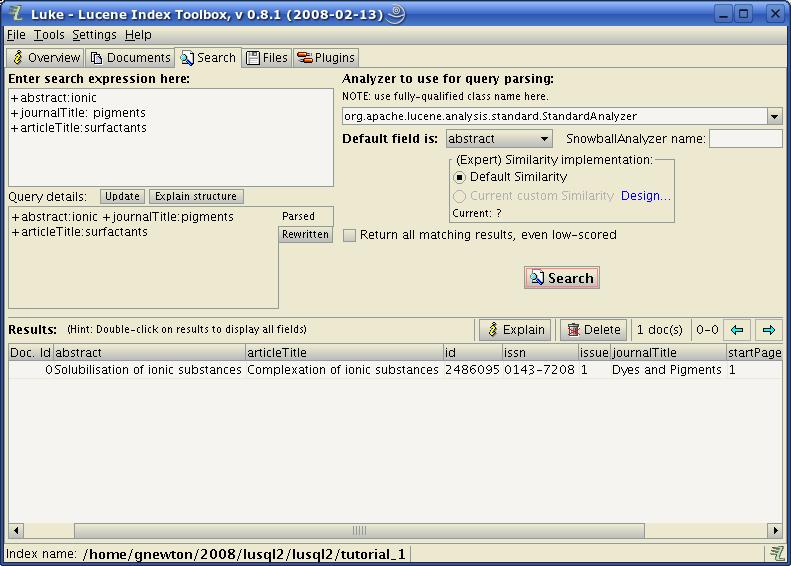
\includegraphics[height=\textwidth]{images/luke_1_3.png}
    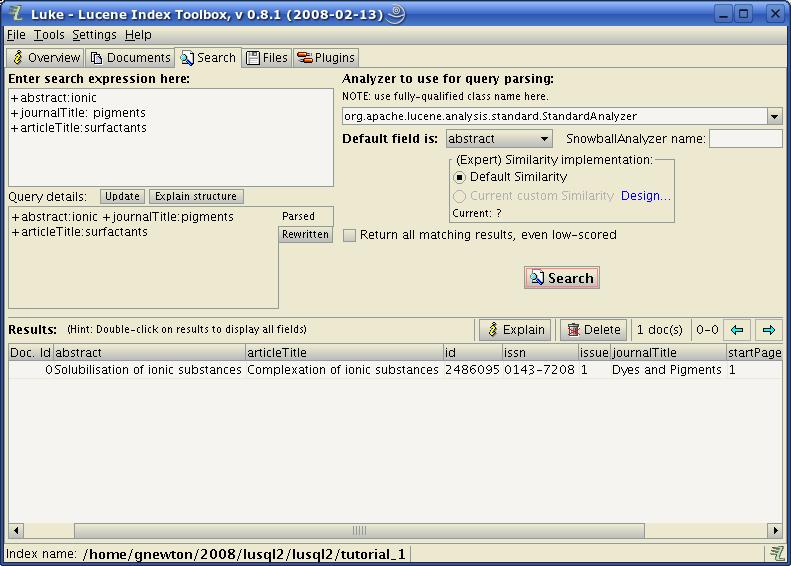
\includegraphics[width=\textwidth]{images/luke_1_3.png}
  \end{center}
  \caption{Example 1 in {\tt Luke}: Search panel}
  \label{luke_1_3}
\end{figure}
%\end{landscape}


\begin{landscape}
\begin{figure}
  \begin{center}
    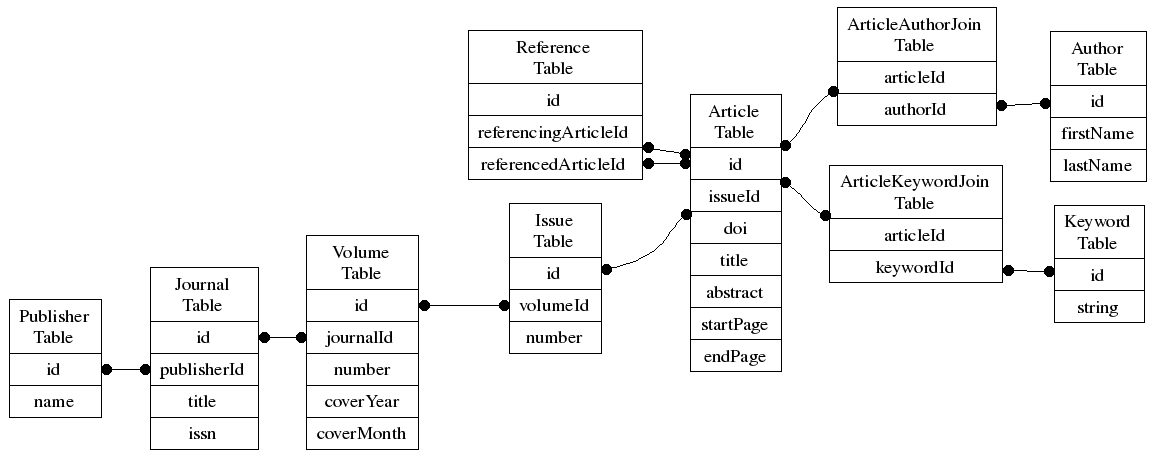
\includegraphics[width=19cm]{dot/tables.png}
%    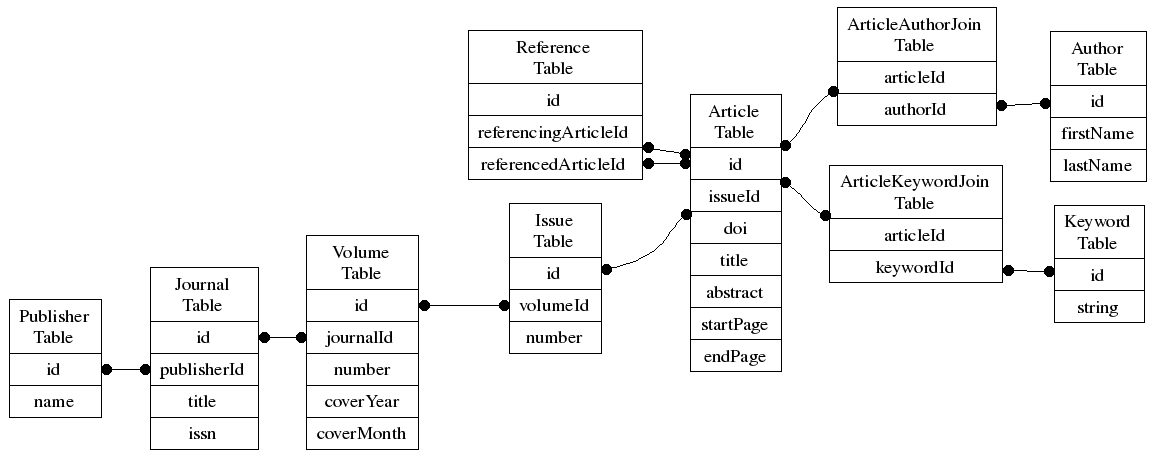
\includegraphics[width=\textwidth]{dot/tables.png}
 %   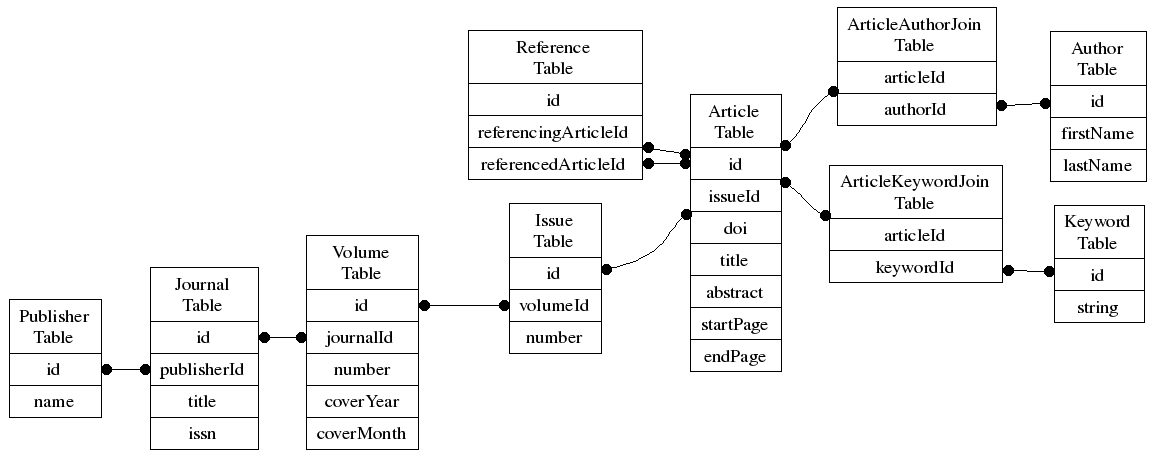
\includegraphics[width=\textheight]{dot/tables.png}
%    \makebox[\textwidth]{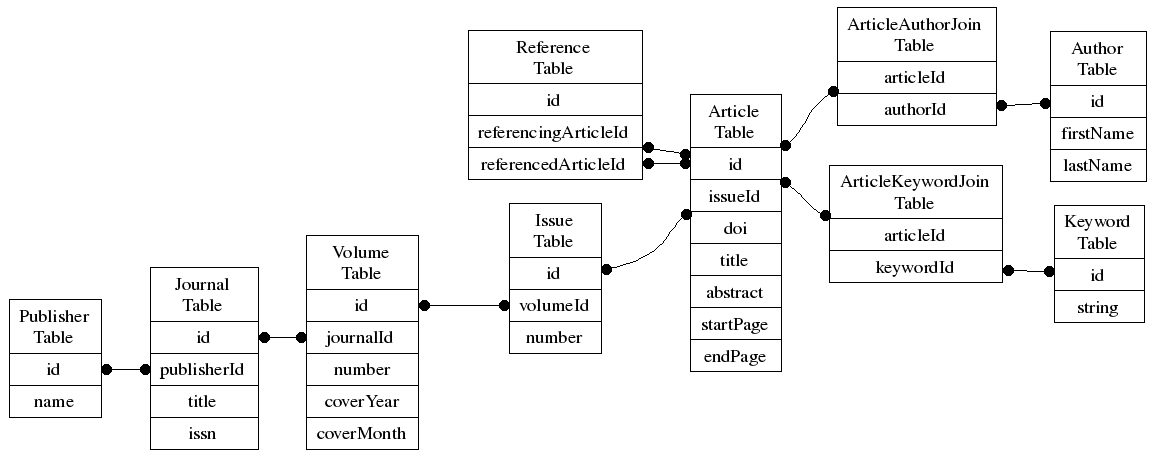
\includegraphics[width=1.15\textwidth]{dot/tables.png}}
  \end{center}
  \caption{Table relationships in Journal Article database}
  \label{tables}
\end{figure}
\end{landscape}



%%%%%%%%%%%%%%%%%%%%%%%%%%%%%%%%%%%%%%%%%%%%%%%%%%%%%%%%%%%%%%%%%%%%


\subsection[Example 2]{Example 2: Multiple tables with joins}
\label{example2}
In this example we use a fairly complex real world example to show some of the
use cases that LuSql can handle.
The database we are going to use is one that would be used to represent
journal articles.
We will use this database for the rest of the examples.
Note that the {\tt Article} table used in these examples is different from the
one used in Example 1.

Figure \ref{tables} shows the example journal article database, with tables
representing publishers, journals, volumes, issues, articles, references
(citations) authors, and keywords. 
The database represents a hierarchy (publisher {\tt hasOneOrMore} journals
{\tt hasOneOrMore} volumes {\tt hasOneOrMore} issues {\tt hasOneOrMore}
 articles) through a series of 1:N relations,
with M:N relations between articles, and authors and keywords respectively,
and a 1:N relationship for articles and references.

For this example, we are interested in the publisher, journal, volume, issue,
article information (publisher name, journal title, journal ISSN, journal
volume, journal volume year, issue number, article id, article title, article
abstract, article start page, article end page).
In order to collect it, the SQL we will use does a series of joins across
these table.

{\small
\begin{lstlisting}[backgroundcolor=\color{grey},language=Bash]
java -jar lusql.jar -q "select  Publisher.name as pub, Journal.title as jo,\
Article.rawUrl as text, Journal.issn, Volume.number as vol,\
Volume.coverYear as year, Issue.number as iss, Article.id as id,\
Article.title as ti, Article.abstract as ab, Article.startPage as startPage,\
Article.endPage as endPage\
from Publisher, Journal, Volume, Issue, Article \
where Publisher.id = Journal.publisherId and Journal.id = Volume.journalId \
and Volume.id = Issue.volumeId and Issue.id = Article.issueId" \
-c "jdbc:mysql://dbhost/db?user=ID&password=PASS" \
-n  50000 -l tutorial-2
\end{lstlisting}
}
Appendix \ref{example2-output} shows the output from this command.
You will notice one difference from the output of Example 1: 
{\small
\begin{lstlisting}[backgroundcolor=\color{grey},language=Bash]
.......... 10000 docs    5s                                                                                   
.......... 20000 docs    3s                                                                                   
.......... 30000 docs    4s                                                                                   
.......... 40000 docs    5s                                                                                   
.......... 50000 docs    5s                                                                                   
\end{lstlisting}
}
With the verbose output, LuSql provides a progress indicator and prints out a
period for each 1000 documents it indexes.
It then prints a total and a time to index, for each 10,000 documents indexed.


\subsubsection{Example 2 examined in Luke}
Again, we examine the index with Luke:
\begin{mlist}
\item Figure \ref{luke_2_1} shows the {\tt Overview} panel, showing the 50,000 {\tt
    Document}s have been added.
\item Figure \ref{luke_2_2} shows the {\tt Document} panel, showing the fields
  derived from the SQL join.
\item Figure \ref{luke_2_3} shows a search and two resulting {\tt Documents}. 
  The search reveals an underlying data problem with the original DBMS, as
  these two {\tt Document}s are the same article, with the only difference
  with one having an issue number of {\tt 1} with the other having an issue
  number of {\tt none}.
  Otherwise this index is behaving as expected.
\end{mlist}

%\begin{landscape}
  \begin{figure}
  \begin{center}
 % 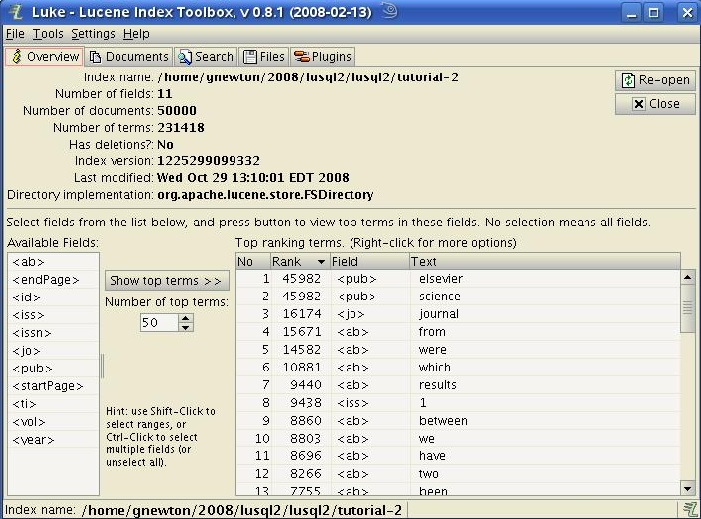
\includegraphics[height=\textwidth]{images/luke_2_1.png}
 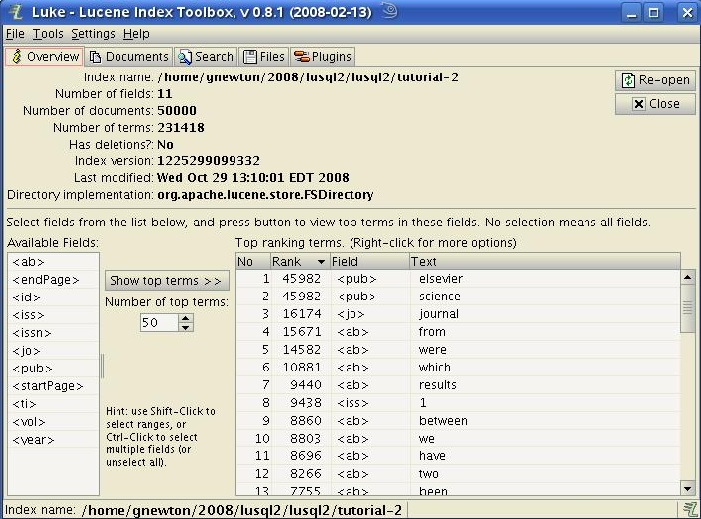
\includegraphics[width=\textwidth]{images/luke_2_1.png}
      \end{center}
  \caption{Example 2 in {\tt Luke}: Overview panel}
\label{luke_2_1}
\end{figure}
%\end{landscape}
%\begin{landscape}
  \begin{figure}
  \begin{center}
%  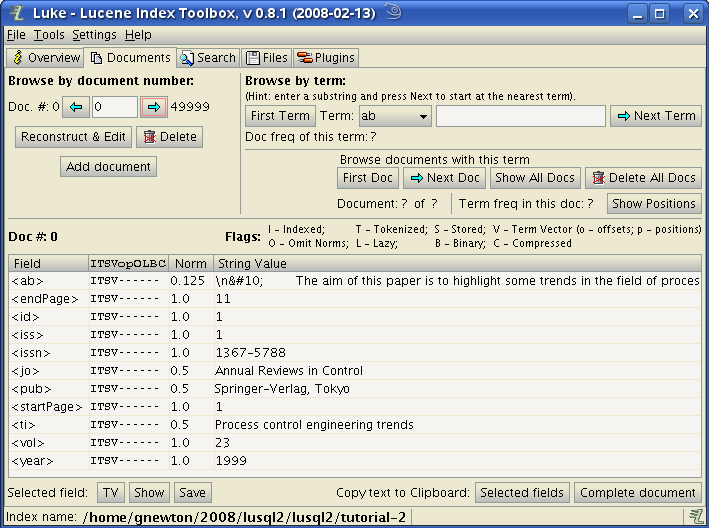
\includegraphics[height=\textwidth]{images/luke_2_2.png}
  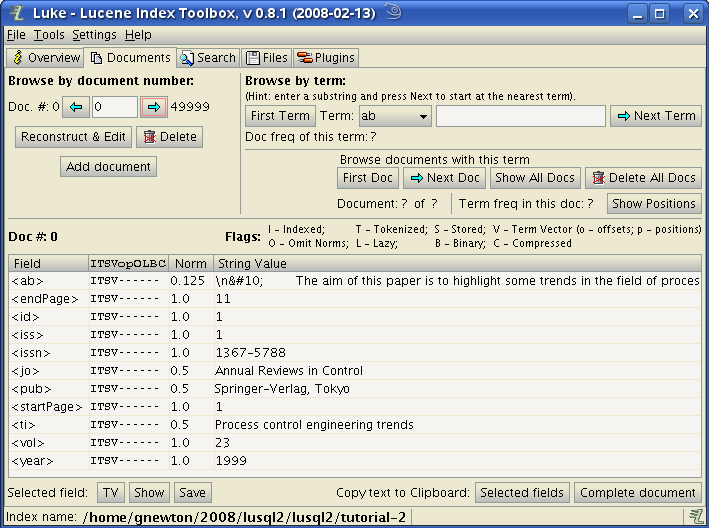
\includegraphics[width=\textwidth]{images/luke_2_2.png}
      \end{center}
  \caption{Example 2 in {\tt Luke}: Documents panel}
\label{luke_2_2}
\end{figure}
%\end{landscape}
%\begin{landscape}
\begin{figure}
  \begin{center}
%    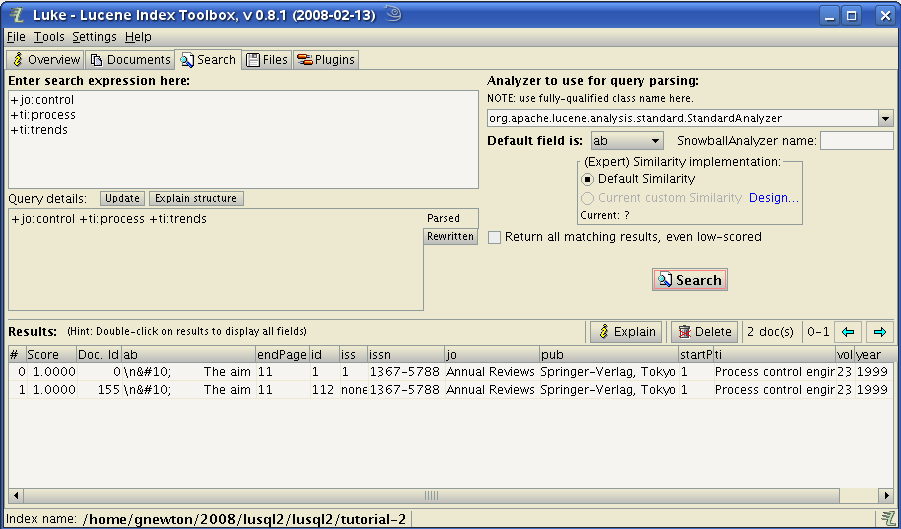
\includegraphics[height=\textwidth]{images/luke_2_3.png}
    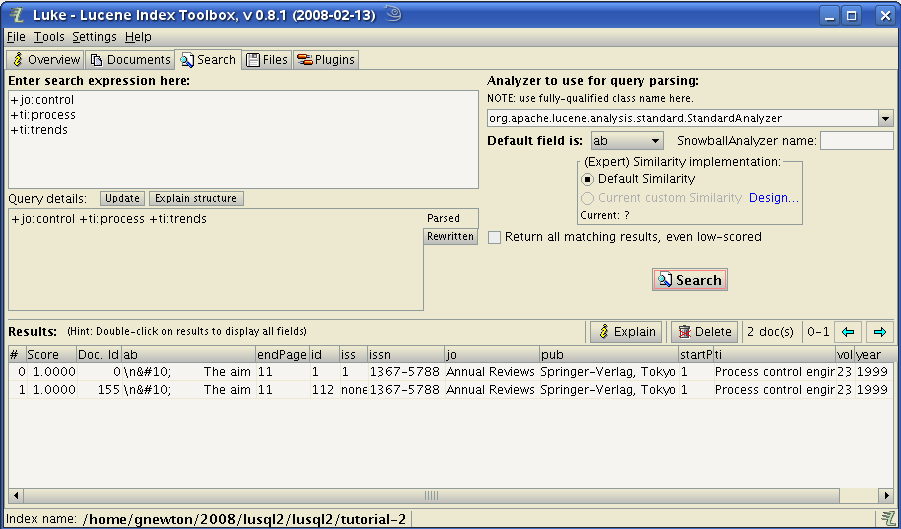
\includegraphics[width=\textwidth]{images/luke_2_3.png}
  \end{center}
  \caption{Example 2 in {\tt Luke}: Search panel}
  \label{luke_2_3}
\end{figure}
%\end{landscape}


\subsection[Example 3]{Example 3: Multiple tables with joins and additional
  subqueries} 
\label{example3}
We continue using the journal article database.
If we were really wanting to create a useful Lucene index for journal
articles, one of the things that would certainly be needed would be the
ability to search articles by authors and/or keywords, or to navigate by
references. 
However, the Lucene index created with Example 2 does not offer this, and
indeed the functionality presented up to now of LuSql does not allow
us to make this sort of index.

LuSql, however, does offer additional functionality to do this sort of thing.
For each {\tt Document}\footnote{Internally, LuSql does not use Lucene {\tt
    Document}s until just before sending the information to be indexed. 
  Instead, LuSql uses its own abstraction for a document, {\tt Doc}, which
  described in Section \ref{doc}.} 
created from the original SQL query, one or more
additional queries can be formulated and run to obtain additional information
from the DBMS and add this to the {\tt Document}. 
These additional queries are constructed by defining a field from the original
query results which is used as a linking key in the additional queries. 

In our example, we want the field {\tt id} from the {\tt Article} table to be used
in SQL queries to get the author, keyword and reference information from their
respective tables.
The relationship between {\tt Article} and both {\tt Author} and {\tt
  Keyword} is many--to--many, with each table having a join table to handle
this relationship ({\tt ArticleAuthorJoin} and {\tt ArticleKeywordJoin},
respectively). 
The relationship between {\tt Article} and {\tt Reference} is a one--to--many.

The queries to select the appropriate authors, keyword and references for a
particular article, say
{\tt Article.id=3453}, would therefor be:
\begin{lstlisting}[backgroundcolor=\color{grey},language=SQL]
select Keyword.string as keyword 
 from ArticleKeywordJoin, Keyword
 where ArticleKeywordJoin.articleId=3453 and
 and ArticleKeywordJoin.keywordId = Keyword.id;

select concat(lastName,', ', firstName) as fullAuthor 
 from ArticleAuthorJoin, Author
 where ArticleAuthorJoin.articleId = 3453 
 and ArticleAuthorJoin.authorId = Author.id;

select referencedArticleId as citedId 
 from Reference 
 where Reference.referencingArticleId = 3453;
\end{lstlisting}


LuSql supports this sort of subquery through an additional command line
parameter {\tt-Q}.
This parameter takes a field from the main query whose value is used as a key
in the subqueries.
In the above example, these would be {\tt Article.id} and 3453, respectively.

When constructing the SQL query, the metavariable {\tt @} is used in the
place where the key value literal would be used.
When LuSql is run, the {\tt @} is replaced with the value of the
field name ({\tt fieldName}) from each {\tt Document} object and any fields
returned (via records) are added to the {\tt Document}. 



Here is how the {\tt -Q} parameters would look like in our example (just add
the below to the LuSql command shown in Example 2, Section \ref{example2}):

\begin{lstlisting}[backgroundcolor=\color{grey},language=SQL]
 -Q "id|select Keyword.string as keyword from ArticleKeywordJoin, Keyword\
  where ArticleKeywordJoin.keywordId=@\ 
  and ArticleKeywordJoin.articleId = Keyword.id"\
 -Q "id|select concat(lastName,', ', firstName) as fullAuthor\
  from ArticleAuthorJoin, Author where ArticleAuthorJoin.articleId = @\
  and ArticleAuthorJoin.authorId = Author.id"\
 -Q "id|select referencedArticleId as citedId\
  from Reference where Reference.referencingArticleId = @"
\end{lstlisting}

Note that the {\tt concat(lastName,', ', firstName)} construct used in the
author query is a MySQL specific function\footnote{
\url{http://dev.mysql.com/doc/refman/5.0/en/string-functions.html}{function\_concat}}.

The {\tt -Q} parameter has the following three variants:
\begin{mlist}
\item {\tt -Q "fieldName|SQL"} --- as per the above example.
\item {\tt -Q "fieldName|NNN|SQL"}
\item {\tt -Q "fieldName|NNN NNN...NNN|SQL"}
\end{mlist}

In the first variant, the {\tt NNN} is left out altogether, and the {\tt NNN} for all
fields for this query are taken from the default value or the value set by the
global {\t -I} (see Section \ref{nnn}).
In the second form, the  {\tt NNN} is the Lucene {\tt Field} index/store/term vector
attributes for all fields returned by the subquery.
In the third form, there is a corresponding {\tt NNN} for each of the fields.



Appendix \ref{example3-output} shows the output for Example 3.

\subsubsection{Example 3 examined in Luke}
Here we will briefly look at the index using Luke.
In Figure \ref{luke_3_1} we can see a document showing the additional fields
added by the {\tt -Q} subqueries ({\tt author, citeId, keywords}).
  \begin{figure}
  \begin{center}
 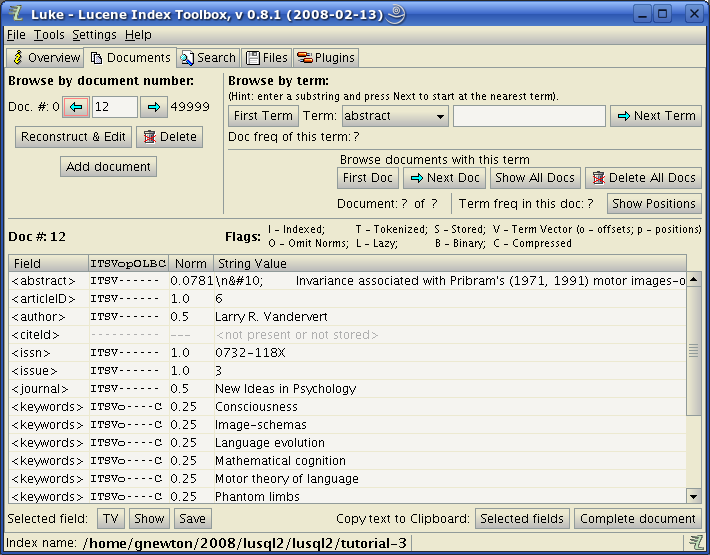
\includegraphics[width=\textwidth]{images/luke_3_1.png}
      \end{center}
  \caption{Example 3 in {\tt Luke}: Documents panel}
\label{luke_3_1}
\end{figure}

%% {\tt 
%% -Q  "id:select Keyword.string as keyword 
%%  $\backslash$\newline
%% from ArticleKeywordJoin, Keyword
%%  $\backslash$\newline
%%  where ArticleKeywordJoin.articleId=@
%%  $\backslash$\newline
%% ArticleKeywordJoin.authorId = Keyword.id"
%% }

%\end{landscape}



\subsection[Example 4]{Example 4: Multiple tables with joins, additional
  queries and filter}
\label{example4}
We continue using the journal article database.
In our journal article database, the article {\em metadata} is kept in the
database, but the full-text of the article is kept in the filesystem in a text
file (extracted from the PDF or supplied by the publisher).
The convention for the path of this file is:\\
{\tt issn/volumeNumber/issueNumber/start-page/arbitraryFileName.txt.gz}.
The field {\tt Article.rawUrl} contains this path, less the {\tt .gz} suffix,
as the files are compressed to save disk space.
So, to create an index that would allow search of the full-text as well as the
metadata, we need to get the full-text content from the filesystem into the 
Lucene index.

LuSql provides a plugin mechanism that allows for arbitrary manipulation of
{\tt Doc}s after they are populated from the database, after any 
{\tt  -Q} additional queries, and before the {\tt Doc} is indexed.
Section \ref{filter} describes how to implement filters ({\tt
  DocFilters}), and Appendix \ref{filterSource} shows the implementation
that we use here to construct the file path, open and un--gzip the file,
read the text from the file into a {\tt String} then add this string 
to the {\tt Doc}, with {\tt Field.Index.TOKENIZED,
Field.Store.YES,\footnote{In a real example, the full-text would likely, not be
  stored, especially in very large collection indexes. In this case, the
  full-text is stored so it can be perused using Luke} Field.TermVector.YES}). 


As this example uses both a filter and subqueries, this may be a good time to
describe the order in which these various things occur in LuSql.
Below is simple pseudocode describing the process:

\begin{lstlisting}[backgroundcolor=\color{grey}]
   foreach resultSet
   {
       make Doc From ResultSet;
       run SubQueries;
       run Filter;
       convert Doc to Lucene Document;
       add Document To Lucene Index;
   }
   run Filter.onDone;
   close Lucene and JDBC Connection;
   optimize Lucene index;
\end{lstlisting}

Appendix \ref{filterSource} shows a filter which implements what we described
above to index the filesystem full-text.
The {\tt -f} command line parameter indicates the filter class to use. 
Append the following text to the command line from Example 3,
Section \ref{example3}) to use the filter we have implemented:
{\small
\begin{lstlisting}[backgroundcolor=\color{grey}]
 -f ca.nrc.cisti.lusql.example.FileFullTextFilter   
\end{lstlisting}
}

Appendix \ref{example4-output} shows the output from this invocation of LuSql.


\subsubsection{Example 4 examined in Luke}
Here we will briefly look at the index using Luke.
In Figure \ref{luke_4_1} we can see a document showing the additional field
added by the filter ({\tt fulltext}.
  \begin{figure}
  \begin{center}
 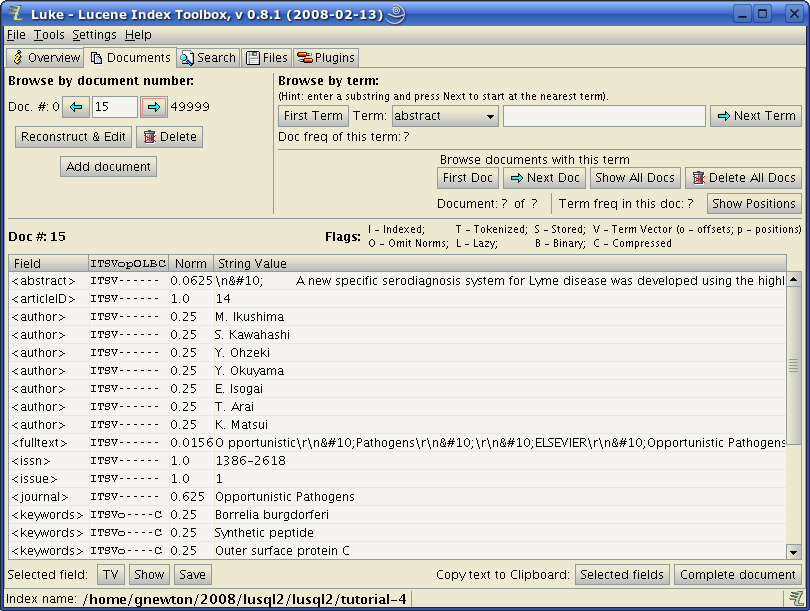
\includegraphics[width=\textwidth]{images/luke_4_1.png}
      \end{center}
  \caption{Example 4 in {\tt Luke}: Documents panel}
\label{luke_4_1}
\end{figure}
